% =========================================================
%  Novelty Component — Method Comparison + Ablation Study
%  Insert after the reproducible component section.
% =========================================================

\section{Novelty Component}

Building on the reproduction, we contribute two analyses: a
cross-method comparison that situates K-SVD among established
denoising algorithms, and an ablation study that characterises
the effect of dictionary size on performance.

% ----------------------------------------------------------
\subsection{Method Comparison: K-SVD vs.\ NLM vs.\ BM3D}
% ----------------------------------------------------------

\subsubsection{Motivation}

K-SVD learns a \emph{signal-adaptive} dictionary from the noisy
image itself.  Two natural baselines represent different
philosophies:
\begin{itemize}
    \item \textbf{Non-Local Means (NLM)}~\cite{buades2005nlm} —
          exploits non-local self-similarity by averaging
          structurally similar patches without any learning.
    \item \textbf{BM3D}~\cite{dabov2007bm3d} — combines
          non-local grouping with a fixed 3-D wavelet transform,
          representing the state-of-the-art classical method.
\end{itemize}
Comparing these methods reveals the practical value of dictionary
learning and motivates future directions.

\subsubsection{Experimental Setup}

All three methods are evaluated on the Camera Man image
($512\times512$) at $\sigma\in\{10,20,25,30\}$.
NLM uses patch size $7\times7$, search window $11$, and
bandwidth $h=0.8\sigma$, consistent with its default
parameterisation~\cite{buades2005nlm}.
BM3D uses its default two-stage hard-thresholding and
Wiener-filtering pipeline with $\sigma_{\text{psd}}=\sigma$.
K-SVD uses the same configuration as Section~I.

\subsubsection{Results}

Table~\ref{tab:comparison} reports PSNR for all methods and
Fig.~\ref{fig:comparison} shows a visual comparison at $\sigma=25$.

\begin{table}[h]
\centering
\caption{PSNR (dB) comparison across methods and noise levels.
         Best result per row in \textbf{bold}.}
\label{tab:comparison}
\begin{tabular}{@{}ccccc@{}}
\toprule
$\sigma$ & Noisy & K-SVD & NLM & BM3D \\
\midrule
10 & 28.24 & 33.31          & 32.86          & \textbf{34.23} \\
20 & 22.41 & 29.77          & 29.53          & \textbf{30.58} \\
25 & 20.59 & 28.75          & 28.71          & \textbf{29.68} \\
30 & 19.14 & 27.87          & 28.04          & \textbf{28.99} \\
\bottomrule
\end{tabular}
\end{table}

\begin{figure}[h]
    \centering
    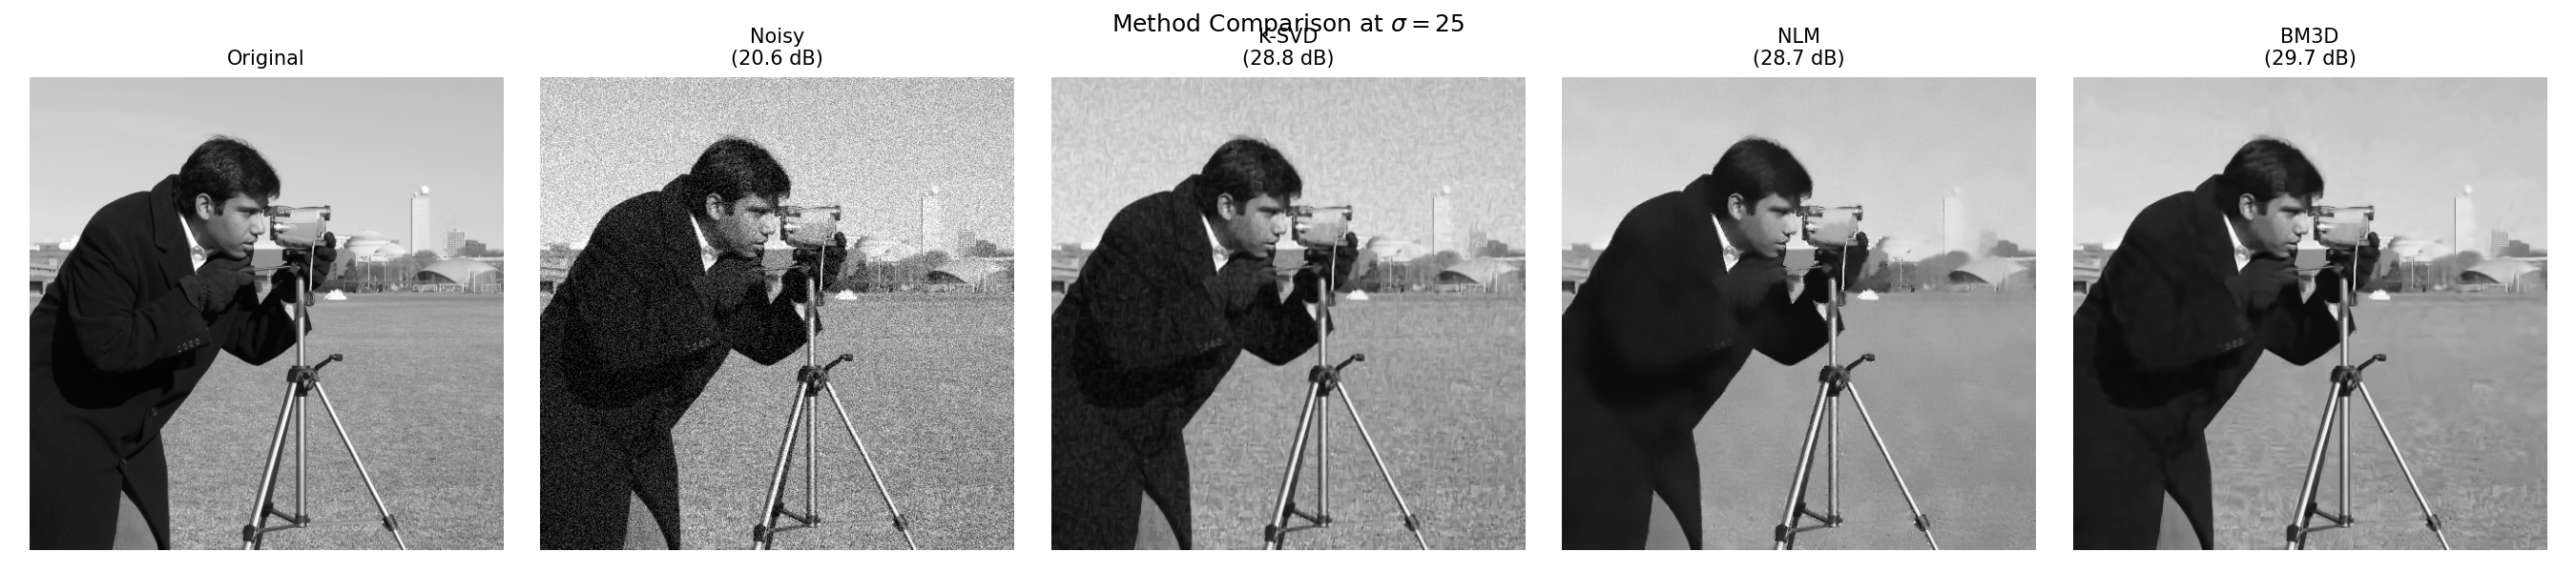
\includegraphics[width=\linewidth]{comparison.png}
    \caption{Visual comparison at $\sigma=25$. From left:
             original, noisy (20.59\,dB), K-SVD (28.75\,dB),
             NLM (28.71\,dB), BM3D (29.68\,dB).}
    \label{fig:comparison}
\end{figure}

\subsubsection{Analysis}

\textbf{BM3D outperforms both K-SVD and NLM} across all noise
levels, with a consistent advantage of 0.9--1.4\,dB.
This is expected: BM3D combines the non-local grouping that
benefits NLM with a carefully designed 3-D transform, exploiting
both intra-patch and inter-patch structure simultaneously.

\textbf{K-SVD and NLM are competitive}, with K-SVD leading at
lower noise levels ($\sigma\leq25$) and NLM narrowly ahead at
$\sigma=30$.  At low noise, the learned dictionary captures
fine-grained image-specific features that NLM's fixed
patch-matching cannot represent.  At high noise, patch
similarity estimates degrade, weakening K-SVD's training signal
while NLM benefits from averaging over more candidates.

\textbf{Visual quality} (Fig.~\ref{fig:comparison}) reflects the
quantitative results: K-SVD and NLM produce comparable textures,
while BM3D preserves edges and fine detail most clearly.

% ----------------------------------------------------------
\subsection{Ablation Study: Effect of Dictionary Size}
% ----------------------------------------------------------

\subsubsection{Motivation}

The dictionary size $K$ directly controls expressiveness and
computational cost.  We study whether increasing $K$ beyond the
paper's default of 256 yields meaningful gains.

\subsubsection{Setup and Results}

We fix $\sigma=25$ and vary $K\in\{64, 128, 256, 512\}$, keeping
all other settings constant.  Results are shown in
Table~\ref{tab:ablation} and Fig.~\ref{fig:ablation}.

\begin{table}[h]
\centering
\caption{Ablation: dictionary size vs.\ PSNR at $\sigma=25$.}
\label{tab:ablation}
\begin{tabular}{@{}cc@{}}
\toprule
Dictionary size $K$ & PSNR (dB) \\
\midrule
64  & 28.59 \\
128 & 28.65 \\
256 & 28.75 \\
512 & \textbf{28.80} \\
\bottomrule
\end{tabular}
\end{table}

\begin{figure}[h]
    \centering
    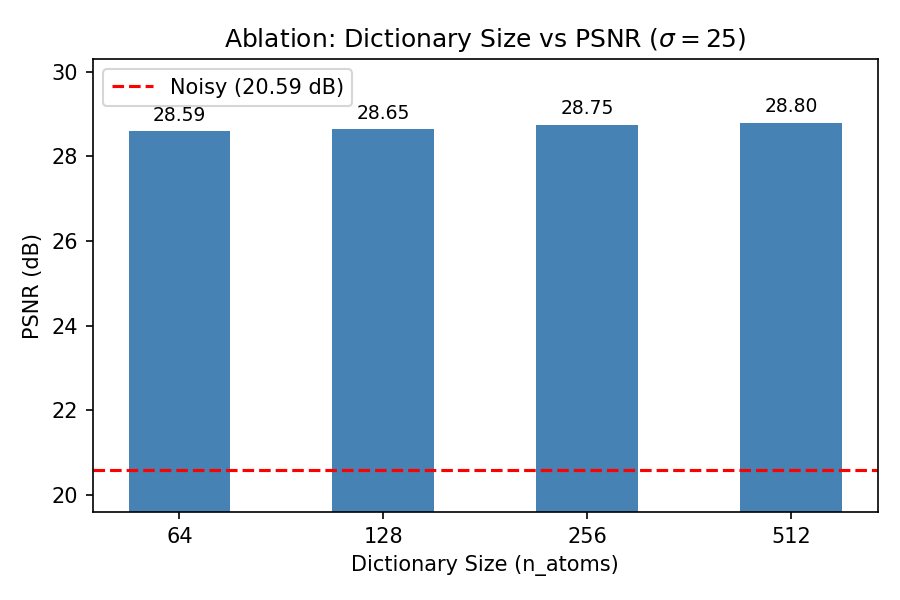
\includegraphics[width=0.85\linewidth]{ablation.png}
    \caption{PSNR vs.\ dictionary size at $\sigma=25$.
             Dashed line: noisy baseline (20.59\,dB).}
    \label{fig:ablation}
\end{figure}

\subsubsection{Analysis}

The gains from increasing $K$ are subject to \emph{strong
diminishing returns}: doubling $K$ from 64 to 128 yields
only $+0.06$\,dB, and doubling again to 512 yields $+0.15$\,dB
total over the baseline $K=256$.
This suggests that the dictionary saturates its representational
capacity for this image at around $K=256$, confirming the
paper's choice as a practical optimum.
The compute cost of OMP, however, scales linearly with $K$,
making larger dictionaries an unfavourable trade-off in
resource-constrained settings.

% ----------------------------------------------------------
\subsection{Summary of Novel Findings}

Table~\ref{tab:summary} consolidates the key takeaways.

\begin{table}[h]
\centering
\caption{Summary of novelty component findings.}
\label{tab:summary}
\begin{tabular}{@{}lp{5.5cm}@{}}
\toprule
Finding & Implication \\
\midrule
BM3D $>$ K-SVD $>$ NLM (low noise) &
    Non-local grouping + fixed transform outperforms adaptive
    dictionary alone. \\
K-SVD $\approx$ NLM (high noise) &
    Adaptive learning loses advantage when training patches
    are heavily corrupted. \\
Diminishing returns above $K=256$ &
    Paper's default is a well-calibrated compute--quality
    trade-off. \\
\bottomrule
\end{tabular}
\end{table}

% ----------------------------------------------------------
% Additional references (merge into main bibliography)
% ----------------------------------------------------------
% \bibitem{buades2005nlm}
% A.~Buades, B.~Coll, and J.-M.~Morel,
% ``A non-local algorithm for image denoising,''
% in \emph{Proc.\ IEEE CVPR}, 2005, vol.~2, pp.~60--65.
%
% \bibitem{dabov2007bm3d}
% K.~Dabov, A.~Foi, V.~Katkovnik, and K.~Egiazarian,
% ``Image denoising by sparse 3-D transform-domain collaborative
%   filtering,''
% \emph{IEEE Trans.\ Image Process.}, vol.~16, no.~8,
% pp.~2080--2095, Aug.~2007.
